\section{Чтение и хранение страниц Wikipedia}

Исследования, описанные в~этой работе, выполнялись на~объектно-ориентированном языке Java.
Он обеспечивает кросплатформенную переносимость продукта
и позволяет использовать наиболее перспективные инструменты из области обработки естественного языка (Natural Language Processing (NLP)\cite{textminingsurvey}).
Помимо этого, известны готовые библиотеки для~обработки Wikipedia, созданные на~этом языке.

\subsection{Формат базы данных Wikipedia}

Рассмотрим формат хранения материала свободной энциклопедии, 
как он опубликован на основном сайте проекта \cite{download}. 
Текст каждой статьи проходит кодирование на~двух уровнях:

\begin{enumerate}

\item {
XML-кодирование, задающее разделение статей внутри одного общего
файла с~указанием идентификатора статьи, возможного перенаправления и~пр.
}

\item{
Кодирование с~использованием специальной разметки Mediawiki (см. \ref{sec:wiki_markup}),
позволяющей задать заголовки, ссылки и~пр.
}

\end{enumerate}

\subsection{XML-кодирование}

XML --- это распространённый формат хранения иерархических массивов данных, 
широко используемый в~сфере Интернет-технологий или в~мире корпоративного ПО. 
Для~многих языках программирования доступны различные библиотеки, 
выполняющие разбор XML-разметки. 
В~основном они делятся на~две группы: 

\begin{enumerate}

\item{
DOM(Document Object Model) --- 
это удобный программный интерфейс доступа к~XML-документу, 
представляющий данные в~виде дерева, где каждому элементу разметки сопоставляется узел таким образом, 
что если элемент $a$ вложен в~элемент $b$ в~XML-документе, то в~получившемся дереве узлы, соответствующие этим элементам, 
будут связаны отношением ``родитель-потомок'' \cite{dom} .
Основной недостаток этого метода заключается в~том, что он подразумевает хранение полученного дерева в~оперативной памяти, 
что в~случае файлов такого размера, как архив Wikipedia, недопустимо.
}

\item {
SAX (Simple API for XML) --- 
это метод последовательного чтения XML-документа \cite{sax}. 
При~его использовании обработчик последовательно читает данные из~XML-файла и по~мере нахождения новых элементов разметки сообщает об~этом вызвавшему приложению, 
используя клиентские функции обратного вызова\cite{callback}. 
Таким образом, приложение-клиент SAX-парсера может получить полную информацию о~содержимом и структуре документа,
не~загружая его целиком в~память. 
Однако и у~этого метода есть свои недостатки. 
Например, если нужно получить содержимое элемента, который находится в~конце файла, придётся обработать все предшествующие элементы, 
что при~размерах документа, сравнимых с~размерами архива  Wikipedia, 
очень трудоёмко.

}

\end{enumerate}

Учитывая возможность обрабатывать с помощью SAX-парсеров объемные XML-документы, 
для~реализации был выбран именно этот метод, несмотря на некоторые его недостатки.

\subsection{Описание формата архива Wikipedia}

Как говорилось выше, архив  базы данных Wikipedia --- это запакованный XML-файл, 
размер которого в~распакованном виде составляет порядка 36Г~Б
При~ознакомительном изучении архива и из~XML-метасхемы \cite{schema} видно, 
что статьи сохранены в~виде тэгов ``page" верхнего уровня. 
Каждый из~них содержит следующие вложенные теги:

\begin{itemize}
\item{{\it title} --- заголовок, уникальный в~рамках всего множества статей;}
\item{{\it id} --- уникальный идентификатор статьи (положительное целое число);}
\item{{\it revision} --- описание последнего изменения статьи (дата, автор);}
\item{{\it text} --- последняя версия текста статьи.}
\end{itemize}

\begin{center}
\textit{Фрагмент дампа английской версии Wikipedia от 02.09.2011.}
\end{center}
\begin{verbatim}
.....

  </page>
  <page>
    <title>Alchemy</title>
    <id>573</id>
    <restrictions>move=:edit=</restrictions>
    <revision>
      <id>447633392</id>
      <timestamp>2011-08-31T10:25:31Z</timestamp>
      <contributor>
        <username>William M. Connolley</username>
        <id>8072</id>
      </contributor>
      <minor />
      <comment>[[Help:Reverting|Reverted]] edits by
	 [[Special:Contributions/115.64.84.154|115.64.84.154]] 
([[User talk:115.64.84.154|talk]]) to last version by 
Car Henkel</comment>
      <text xml:space="preserve">{{Redirect|Alchemist}}
{{Other uses}}

[[File:Raimundus Lullus alchemic page.jpg|thumb|right|Page from
 alchemic treatis
e of [[Ramon Llull]], 16th century]]
'''Alchemy''' is an ancient [[tradition]], the primary objective of 
which was the creation of the mythical &quot;[[philosopher's stone]]
,&quot; which was said to be capable of turning [[base metal]]s into 
[[gold]] or [[silver]], and also

.......
\end{verbatim}

Некоторые статьи, называемые переадресатами, не~содержат текста и служат только для~перенаправления на~другие статьи. 
Это используется в~случае, когда существует несколько возможных названий понятия, 
описываемого в~статье, и по всем ним у~пользователя должна быть возможность перейти к~оригиналу.
В~этом случае тег ``page" содержит внутри себя тег ``redirect'', 
а в~теге ``text'' указан заголовок оригинальной статьи.

В~рамках данной работы основными требованиями к~компоненту, 
отвечающему за~обработку архива, были гибкость и возможность доступа к произвольному участку документа.
Необходимость в~последнем вызвана тем, что:

\begin{itemize}

\item{
Произвольный доступ нужен для параллельной обработки;
}

\item{
При~исключительной ситуации, когда  обработчик некорректно завершает свою работу, 
и нет~возможности установить указатель на~место в~файле, где произошла ошибка,
необходимо начинать обработку всего архива сначала, что очень трудоёмко.
}

\end{itemize}

Предполагая большое количество компонентов, требующих функцию чтения архива Wikipedia,
было принято решение определить следующую архитектуру XML-парсера (рис. \ref{uml:ru.tsu.inf.atexant.dump}):

\begin{enumerate}

\item{
Объект ``parser'' класса ``WikipediaParser'' запускает SAX-парсер, 
который передаёт оповещения о~встреченных XML-элементах и их~содержимом.
}

\item {
Этот объект предварительно конфигурируется другим объектом --- обработчиком статей,
 реализующим интерфейс ``AbstractWikipediaPageHandler'', 
содержащим метод handle(WikipediaPage).
}

\item{
``Parser'' при~прочтении целиком тега ``page'' создает объект ''WikipediaPage'', 
заполняет необходимые поля и передает его обработчику статей.
}

\end{enumerate}




Таким образом, была получена универсальная система чтения архива, 
для использования которой достаточно реализовать простой интерфейс с обработкой одного объекта-страницы.
Для~решения проблемы произвольного доступа к~файлу была создана ``обертка'' для стандартного потока ``InputStream'', которая:

\begin{figure}
\begin{center}
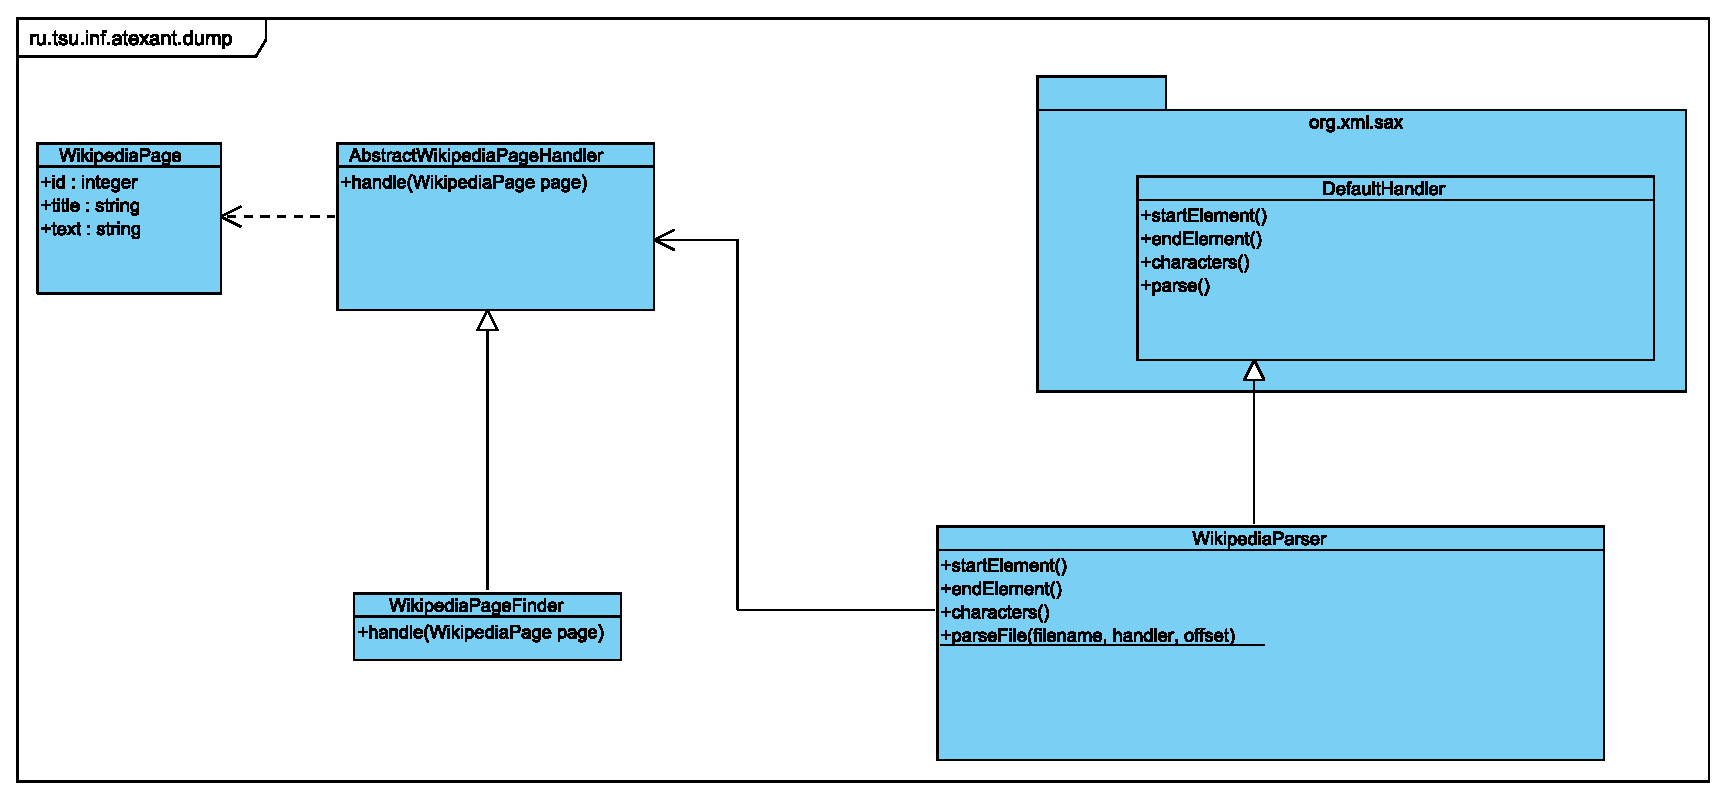
\includegraphics[scale=0.6]{eps/ru.tsu.inf.atexant.dump.eps}
\caption{Диграмма классов пакета ru.tsu.inf.atexant.dump}
\label{uml:ru.tsu.inf.atexant.dump}
\end{center}
\end{figure}

\begin{enumerate}

\item{
Предоставляет возможность определения сдвига в~байтах от~начала файла XML-документа.
}

\item {
Если заданный сдвиг не~указывает на начало тега ``page'', 
то пропускает все байты, 
вплоть до следующего его упоминания.
}

\item{
Самостоятельно “оборачивает" предоставляемые потоком данные в~корневой тег.
}

\end{enumerate}

Последние два пункта нужны для того, чтобы содержимое сформированного потока являлось~бы допустимым XML-кодом.
В~результате была реализована возможность обрабатывать файл-дамп с~произвольным сдвигом от~его начала, 
что значительно увеличило удобство использования этого компонента.  

\subsection{Сопутствующие задачи}

По причине разнородности задач, принятых для~исследования в~рамках настоящей работы,
были решены некоторые вспомогательные подзадачи, которые хоть и не~имеют прямого отношения к~DM, 
но их решение важно для~работы в~целом.

\subsubsection{Разметка Mediawiki}
\label{sec:wiki_markup}

Текст статей Wikipedia включает в~себя помимо основного содержания элементы специальной разметки, которые позволяют \cite{wikimarkup}:

\begin{enumerate}

\item{Управлять внешним видом блоков текста (размер/тип шрифта, цвет, отступ и~т.~п.).}
\item{Определять структуру документа (таблицы, вложенные списки, оглавления).}
\item{Выделять некоторые части текста как ссылки на~другие статьи.}

\end{enumerate}

Поскольку эта разметка содержит одновременно и элементы форматирования внешнего вида,
несущественные для~интерпретации текста, и элементы, значимые при~обработке,
необходим компонент, способный выполнять фильтрацию ненужных элементов форматирования
и передавать обработанные данные в~абстрактный унифицированный интерфейс 
по~ аналогии с~тем, как это делалось при~разборе XML.
В~качестве решения этой проблемы было предложено использовать библиотеку 
JWPL (Java Wikipedia Library)\cite{jwpl}, 
которая содержит инструменты для~работы с~разметкой Mediawiki\cite{wikimarkup} 
и дает программный доступ к~отдельным ее элементам, таким~как:

\begin{itemize}

\item {список ссылок на другие статьи;}
\item{вложенные списки и оглавления;}
\item{Таблицы и интерфейс для~их~обработки;.}

\end{itemize}

Для~того, чтобы обеспечить изоляцию деталей библиотеки, 
в~соответствии с~паттерном ``шлюз'' \cite{patternGateway} был создан класс, 
предоставляющий остальным компонентам системы доступ к~библиотеке.

\subsubsection{Хранение в~базе данных}

Формат архива Wikipedia, рассмотренный выше, не~предназначен и неудобен для произвольного доступа к~определенным статьям. 
Чтобы найти текст статьи по~её~названию, идентификатору или ключевым словам,
необходимо обработать весь архив.

Для~обеспечения более удобного доступа было принято решение сохранять необходимую информацию в~БД,
которая кроме хранения информации предоставляет инструменты для~её~обработки и поиска.

В~качестве такой БД изначально была выбрана свободная реляционная 
СУБД MySQL, представляющая собой удобный инструмент для~решения поставленных задач 
с~возможностью выполнения индексации и хорошей масштабируемостью, 
но с~недостаточными инструментами для~полнотекстового поиска \cite{mysql}.
Из-за последнего недостатка было решено ограничиться хранением и индексированием в~MySQL следующей информации о~страницах:

\begin{itemize}

\item{числового идентификатора;}
\item {заголовка;}
\item {в~случае перенаправления, заголовка и идентификатора базовой статьи;}

\item {
Сдвига в~байтах от~начала архива-исходника, 
где расположена страница.
}

\end{itemize}

Другими словами, для~получения текста определенной страницы, например по~её~названию,
нужно найти строку в~таблице статей с фильтром по~названию,
получить сдвиг для данной статьи, ее идентификатор, и, 
воспользовавшись описанным выше компонентом для~разбора архива, найти нужную статью, 
указав необходимый сдвиг.

Для~более удобной работы с БД, используя паттерн проектирования Data Mapper\cite{patternMapper}, 
был создан компонент для сохранения и поиска страниц Wikipedia в~базе.

В~ходе дальнейших исследований предполагается изучение более производительных БД, таких~как 
Lucene \cite{lucene} и 
MongoDB \cite{mongodb}. 
Они лучше приспособлены для~поиска в~массивах текстов подобного размера.

\section{Обработка естественного языка}

Обработка естественного языка (Natural Language Processing (NLP))\cite{textminingsurvey} --- 
одна из~самых важных областей для исследований, сопутствующих извлечению информации из текстов.
Основная цель NLP состоит в~повышении качества разбора естественных языков машинами.
Из~основных направлений NLP стоит упомянуть следующие:

\begin{itemize}

\item {Морфологический анализ текста --- определение частей речи для~отдельных слов текста;}
\item {Лемматизация --- приведение слов текста к~нормальной форме (инфинитив, ед.~число, и~т.~д.);}
\item {Синтаксический анализ --- нахождение связей между членами предложений.}

\end{itemize}

Задачи, связанные с~каждым из~упомянутых разделов NLP, 
являются предметом отдельных научных исследований и выходят за~рамки настоящей научной работы.
В~значительной мере они были проведены исследователями Стэнфордского университета. 
Для~решения проблем, связанных с обработкой естественных языков, была использована библиотека  Stanford CoreNLP,
реализующие известные достижения.

\subsection{Stanford CoreNLP}
\label{st_corenlp}

Пакет Stanford CoreNLP --- это один из~самых развитых инструментов для~работы с~естественными языками \cite{corenlp}, 
первая версия которого датируется 1~ноября~2010~г.
Он является набором классов на языке Java, предоставляющих интерфейсы для~решения многочисленных проблем NLP. 

В~настоящей работе использовались две подсистемы CoreNLP:

\begin{enumerate}

\item {{\it POS-tagger}, предназначенный для~определения частей речи слов и их~лемматизации.}
\item {{\it Parser}, предоставляющий возможность строить дерево зависимостей членов предложений.}

\end{enumerate}

Основными понятиями пакета CoreNLP являются {\it Аннотации} и {\it Аннотаторы}. 
Для~того, чтобы получить те или иные результаты работы NLP-алгоритмов,
пользователь пакета должен создать объект-документ,
содержащий коллекцию аннотаций для~исходного текста. 
Затем необходимо выбрать Аннотаторы, каждый из~которых решает свою задачу, 
добавляя в~коллекцию соответствующие аннотации, и применить их к~тексту. 
Необходимо учитывать, что некоторые аннотаторы требуют результаты работы некоторых вспомогательных аннотаторов.
Например, аннотатор, ответственный за~лемматизацию, может быть запущен
только в~том~случае, если документ уже был обработан аннотатором частей речи.

Некоторые аннотаторы позволяют разбивать текст на отдельные предложения и слова,
причем аннотации, которые были применены к исходному документу, будут присутствовать и
и в~выделенных его частях. 
Другими словами, если применить к~тексту аннотаторы, разбивающие текст на отдельные слова,
вместе с~аннотатором частей речи, то результаты работы второго аннотатора 
можно получить как для всего текста, так и для отдельных его слов.

Список всех аннотаторов и их аннотаций доступен на~сайте CoreNLP \cite{corenlp}.

\subsection{Способы представления лингвистической информации в~CoreNLP}
\label{sec:corenlp_representation_methods}
Как было сказано выше, в~настоящей работе CoreNLP использовался в~основном для~
определения частей речи и анализа грамматических зависимостей членов предложений.
Если с морфологическим анализом все относительно просто ---
 каждому слову из~текста сопоставляется один из~тегов частей речи, список которых можно найти в~\cite{treebank},
то с~синтаксической частью несколько сложнее.

Базовым способом представления результатов синтаксической части является структура,
которая в~лингвистике имеет название ``грамматика непосредственно составляющих'' (phrase structure grammar). 
Описание её~формата можно найти в~книге ``Синтаксические структуры'' \cite{homsky}.
Это представление является наиболее полным и обоснованным с~точки зрения лингвистики, 
однако несколько неудобным для~анализа связей между отдельными членами предложения.
Для~решения этой проблемы в~пакете CoreNLP существуют инструменты 
для~преобразования грамматики непосредственно составляющих к~более простой форме списка зависимостей членов предложения, 
каждый элемент которого имеет вид:

\begin{verbatim}

<тип зависимости>(<слово1>-<номер слова1>,<слово2>-<номер слова2>).

\end{verbatim}

Причем первое слово в~паре считается главным, а второе --- зависимым.
Список типов зависимостей можно найти в~\cite{dependencies}.

Если построить граф с~вершинами-членами предложений, а в~качестве ребер использовать отдельные зависимости из~полученного списка, 
то этот граф, поскольку у~каждого члена предложения может быть не~более одного управляющего слова, 
очевидно, будет являться деревом. 
Назовём его ``деревом зависимостей предложения''.
Эта форма была выбрана для~дальнейшей работы со~структурой предложения.

Приведем пример работы аннотатора для предложения ``If I had a gun I'd shoot a hole into the sun''.
Его грамматика непосредственно составляющих выглядит следующим образом:

\begin{verbatim}

(ROOT
  (SBAR (IN If)
    (S
      (NP (PRP I))
      (VP (VBD had)
        (NP
          (NP (DT a) (NN gun))
          (SBAR
            (S
              (NP (PRP I))
              (VP (MD 'd)
                (VP (VB shoot)
                  (NP (DT a) (NN hole))
                  (PP (IN into)
                    (NP (DT the) (NN sun)))))))))))).

\end{verbatim}

А его список зависимостей имеет вид:

\begin{verbatim}

mark(had-3, If-1)
nsubj(had-3, I-2)
root(ROOT-0, had-3)
det(gun-5, a-4)
dobj(had-3, gun-5)
nsubj(shoot-8, I-6)
aux(shoot-8, 'd-7)
rcmod(gun-5, shoot-8)
det(hole-10, a-9)
dobj(shoot-8, hole-10)
prep(shoot-8, into-11)
det(sun-13, the-12)
pobj(into-11, sun-13)

\end{verbatim}

Дерево зависимостей изображено на рис. \ref{fig:dependency_tree}.

\begin{figure}
\begin{center}
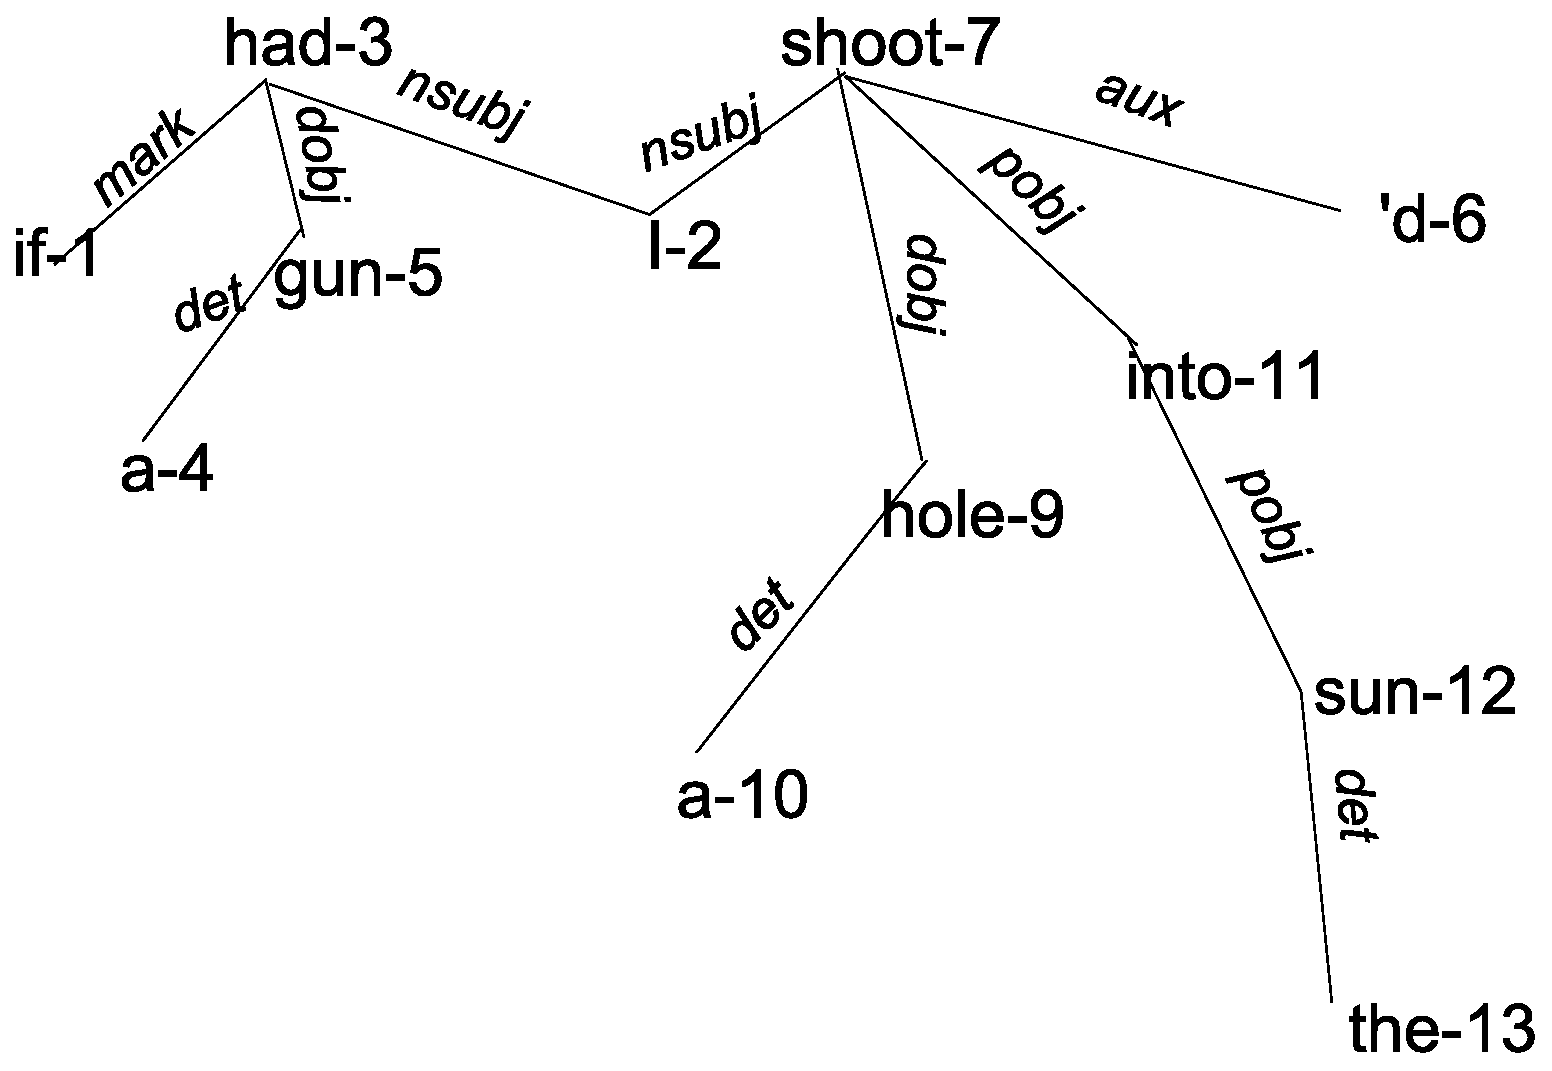
\includegraphics[scale=0.4]{eps/dependency_tree.eps}
\caption{Дерево зависимостей предложения ``If I had a gun I'd shoot a hole into the sun''}
\label{fig:dependency_tree}
\end{center}
\end{figure}

\subsection{Ограничения CoreNLP}

Алгоритмы библиотеки CoreNLP имеют ряд существенных ограничений, о~которых не~стоит забывать, 
рассматривая её как альтернативу при~выборе NLP-пакета.
Одной из проблем может стать то, что CoreNLP в~её~текущей комплектации
предназначена в~основном для работы с английским языком, 
и её адаптация к~лингвистическим особенностям других языков, включая русский,
является нетривиальной задачей, если вообще возможной.

Вторым аспектом, ограничивающим применение CoreNLP, является трудоемкость её алгоритмов. 
При~загрузке всех своих словарей, необходимых для~морфологического анализа, 
структуры CoreNLP могут занять до~одного гигабайта оперативной памяти.
Кроме этого, стоит заметить, что время работы парсера, строящего дерево предложения,
так же оставляет желать лучшего: измерения показали, что для~предложения
из~обычного художественного текста среднее значение времени работы $0.6$~с,
а в~случае сложных предложений может доходить и до~одной секунды.

\section{Оценка близости предложений}

Оценка близости предложений является сегодня одной из~самых важных частей алгоритмов,
 связанных с~классификацией и кластеризацией документов\cite{textminingsurvey}, 
основной частью которых является некая функция оценки близости документов,
которую можно построить на~основе сравнения схожести предложений, их~составляющих.

Также полученную оценку можно использовать для~определения оригинальности
авторства текстов.
Кроме этого, модифицированные методы определения близости пригодны к~использованию и при~поиске по~набору документов.

Сформулируем задачу следующим образом:
введём меру близости, как функцию от~двух аргументов-предложений, отвечающую следующим требованиям:

\begin{enumerate}

\item {
Её~значения находятся в~интервале $[0,1]$.
}

\item {
Если взять значения этой меры для~двух различных пар предложений, 
то большее значение должно соответствовать той паре, которая по~мнению большей группы опрошенных людей считается более близкой по~смыслу.
}

\end{enumerate}

Поскольку вторая часть определения слабо формализована, 
все~алгоритмы построения меры близости носят эвристический характер и не~могут быть строго научно сформулированы.
В~рамках настоящей научной работы был исследован ряд существующих алгоритмов,
и один из~них, выбранный как наиболее перспективный, был реализован.
Кроме этого, качество его работы было оценено, в~том числе на~примере статьи Wikipedia, 
и предложены варианты его~дальнейшего улучшения.

Рассмотренные методы можно разделить на следующие три~типа:

\begin{enumerate}

\item{
Алгоритмы, которые рассматривают предложения и отдельные слова только как символьные строки, 
определяя меру близости на~основе разнообразных статистических методов, 
руководствуясь при~этом только сходством в~написании слов (см. \ref{sec:first_type_algorithm}).
}

\item {
Методы, которые рассматривают слова предложений как~множество понятий в~смысле онтологии.
То~есть алгоритмы этого класса абстрагируются от~написания слов, работая с ними
как с~семантическими единицами\cite{wordnetSim}. 
Этот подход позволяет распознавать синонимы или одни и~те~же~слова, находящиеся в~разных формах,
и на~основе этого делать выводы о~сходстве предложений даже в~тех случаях,
когда алгоритмы первого класса показывают нулевые результаты (см. \ref{sec:second_type_algorithm}).
}

\item {
Алгоритмы, которые  для~определения близости  кроме смыслового значения слов
используют также связи, образованные этими словами в~предложении (см. \ref{sec:third_type_algorithm}).

}
\end{enumerate}

\subsection{Обзор существующих алгоритмов}
\subsubsection{Алгоритмы первого типа}
\label{sec:first_type_algorithm}

Авторы \cite{statisticalSim} сравнивают предложения, 
как упорядоченные списки составляющих их слов, 
причем слова сравниваются только исходя из~эквивалентности их~написания. 
Для~установления степени близости таких двух списков авторы предлагают несколько статистических методов,
начиная от~самых стандартных, таких~как определение отношения пересечения множества слов в~этих списках к~их объединению
или представление списков, как векторы, где близость определяется косинусом угла между ними,
до~более сложных формул, учитывающих порядок слов в~предложении и расстояние между ними.

Преимущество такого подхода состоит в~том, что он прост в~реализации, не требует
сложных дополнительных инструментов, обладает низкой трудоемкостью, и кроме всего прочего,
 полученная реализация не~будет зависеть от языка предложений, 
т.~к. использует только написание слов.
Основным недостатком методов этого типа является то, что они  не~приспособлены к многозначности и полиморфизму естественных языков, 
и, например, в~случае  использования в~двух предложениях слов с~одинаковым смыслом, но с~разным написанием 
значение меры сходства будет близким к нулю.

\subsubsection{Алгоритмы второго типа}
\label{sec:second_type_algorithm}
Для~борьбы с~этими недостатками можно воспользоваться методами, описанными в~\cite{wordnetSim}.
Её~авторы предлагают использовать WordNet --- семантическую сеть для английского языка \cite{wordnet}, 
разработанную в~Принстонском университете для~оценки близости отдельных слов-членов предложения.
Основная суть работы алгоритма состоит в~том, 
что для~исходных предложений строится полный взвешенный двудольный граф, 
%%FIXME:Граф разве может быть полным и двудольным?
%%Да, двудольный граф называется полным, если для каждой пары вершин из разных долей есть ребро (опр. из википедии)
вершинами которого являются отдельные слова каждого из~предложений, 
а вес каждого из~ребер равен значению меры близости слов $Sim_{words}(w_1, w_2)$,
соответствующих вершинам на~концах ребра. 

$Sim_{words}(w_1, w_2)$ --- величина, значения которой также принадлежат интервалу $[0,1]$,
показывает насколько слова $w_1,w_2$ семантически близки.

Результатом работы этого алгоритма является максимальное взвешенное паросочетание на~этом графе, 
находимое венгерским алгоритмом\cite{hungarian}.

То есть в сущности решается задача о назначении\cite{oper_research}, в которой
нужно каждому слову первого предложение поставить в соответствие одно слово из второго,
так, чтобы максимизировать суммарную схожесть всех пар.

Для~того, чтобы итоговая мера близости принадлежала интервалу $[0,1]$ ее нормируют на~вес ребер.

Подобные алгоритмы, сравнивающие не просто близость написания слов, 
но и близость их смысла, могут дать более точные результаты в~случаях, 
когда близость предложений скрыта синонимичными различиями в~написании.

Однако для~их реализации необходимы такие наработки из областей NLP и DM,
как лемматизация слов и семантическая сеть, подобная WordNet\cite{wordnet}.

%% тут можно опять же пересечь с материалом Валентины, поскольку у неё последний разбор был про мегаразвитую сеть понятий.
%%Не, пока пропустим, очень многоэтажно получается.

Кроме того подобные алгоритмы не учитывают роли, которую играют слова в~предложении,
а~так же их отношения, что завышает итоговую меру близости в~случаях,
когда сравниваются предложения со~схожими наборами слов, но с~разным смыслом,
т.~е. с~различиями, заключенными в~синтаксической структуре.

\subsubsection{Алгоритмы третьего типа}
\label{sec:third_type_algorithm}
Третий тип методов призван решить последнюю проблему. 
Алгоритмы этого класса устанавливают меру близости предложений на~основании двух факторов:

\begin{enumerate}

\item{
Близость семантических ролей отдельных членов предложения.
}

\item{
Близость синтаксических отношений, образующих эти предложения.
}

\end{enumerate}

Для~установления величины второго фактора в~этих алгоритмах чаще всего используются
деревья зависимостей предложений, суть которых была изложена выше в~разд.~\ref{st_corenlp}.
Автором были изучены две статьи, описывающие методы, 
использующие в~своих оценках связи между отдельными членами предложений.
В~\cite{weightedDep} предлагается следующий подход:

\begin{enumerate}

\item {
Строятся деревья зависимостей оцениваемых предложений.
}

\item {
Для каждой зависимости $d$ определяется ее  вес $weight(d)$, равный величине,  
зависимой от~расстояния до~корня дерева.
Эта~величина характеризует ``значимость'' конкретной зависимости.
Предполагается, что чем дальше от~корня находятся слова, тем меньше они влияют на~общий смысл предложения. 
Кроме этого, в~весе учитывается тип конкретной связи.
Так, например, связь ``управление'' между глаголом и существительным 
%%FIXME:Тут смысл не очень ясен, что такое тип связи?
%%имеются ввиду типы связи словосочетаний (например управление, согласование, примыкание)
%%это скорее из области лингвистики, но в~целом мне показалось очевидным,
%%что одни и те же слова могут быть связаны по-разному в~зависимости от их ролей.
может быть оценена выше, чем ``согласование'' между именами существительным и прилагательным.
}

\item{
Вводится мера близости отдельных связей, как линейная комбинация
величин близости управляющих и подчиненных слов в~них.
$$d2dSim(d_1,d_2) = \lambda_1 \cdot Sim_{words}(h(d_1),h(d_2)) + \lambda_2 \cdot Sim_{words}(m(d_1),m(d_2)), $$
где $d_1, d_2$ --- пара сравниваемых зависимостей,\\
$h(d_i), m(d_i)$ --- управляющее и подчиненное слова зависимости $d_i$,\\
$Sim_{words}(w_1,w_2)$ --- мера схожести слов, найденная с использованием Wordnet (см. \ref{sec:second_type_algorithm}),\\
а $\lambda_1 + \lambda_2 = 1$.

Далее строится полный двудольный взвешенный граф, в~котором каждая доля соответствует отдельному предложению,
вершинами являются синтаксические связи $d$ этих предложений,
а вес ребер между вершинами разных долей равен описанной выше мере близости
данных связей.
}

\item {
Определяется максимальное паросочетание на~графе,
построенное в предыдущем пункте.
Суть этого шага состоит в том, чтобы найти как можно
больше взаимооднозначных соответствий между зависимостями
сравниваемых предложений.
}

\item {
Вершины-зависимости, для~которых не~были найдены пары,т.е. не~вошедшие в~паросочетание, 
помечаются как ''беспарные''.
Также ''беспарными'' cчитают вершины,  для~которых значения веса ребра из~паросочетания, 
проходящего через них, ниже определенного порога.
Таким образом можно полагать, что ''беспарные'' связи первого предложения это те из них,
для которых не было найдено подходящей по смыслу связи во втором, и наоборот. 
}

\item{
В~качестве меры близости предлагается величина 
$paraphrase(S_1, S_2) = sim(S_1,S_2)/diss(S_1, S_2)$, 
где $sim(S_1, S_2)$ --- это вес максимального паросочетания,
а $diss(S_1, S_2)$ --- это величина, зависящая прямо пропорционально  
от~суммы весов ``значимости'' для~беспарных зависимостей.
}

\end{enumerate}

Предложенный алгоритм учитывает как семантическую, так и синтаксическую составляющую предложений, 
что потенциально позволяет всесторонне оценить искомую меру близости.
Дополнительно авторы статьи предлагают достаточно интересную идею оценки значимости связей
в~зависимости от~их~расстояния до~корня дерева и их~типа.
Подобный подход кажется эмпирически обоснованным, 
поэтому пропуск этого аспекта в~алгоритме,
описанном в~следующей рассмотренной статье, можно считать значительным недостатком.

В~ходе анализа эффективности алгоритма автором был выявлен ряд недостатков,
и по~этой причине было принято решение взять для реализации описанный ниже алгоритм.

Во-первых, следует учесть то, что авторами статьи\cite{weightedDep} изначально были поставлены несколько иные цели. 
Для~них главным был ответ на вопрос, можно ли считать одно из предложений парафразом (пересказом) другого. 
Это несколько более узкая задача,
результаты которой не~всегда могут коррелировать с~близостью предложений.

Во-вторых, ещё одним выявленным недостатком этого метода является примитивность используемого математического аппарата. 

В~частности, можно упомянуть несостоятельность выбора алгоритма паросочетания. 
Предложенный авторами подход может часто находить неоптимальные варианты,
что уменьшает общую эффективность метода. 

В~заключение, для~подсчета итогового коэффициента вероятности что данные предложения
являются парафразами, использовались достаточно примитивные статистические методы,
которые могут давать крайне неточные результаты.

\subsubsection{Алгоритмы третьего типа. Комплексный подход}
\label{sec:complex_algorithm}
Авторы \cite{complexSim} предлагают более комплексный подход, 
суть которого заключается в~декомпозиции задачи
оценивания близости предложений на~подзадачи оценивания более узких аспектов, 
характеризующих их~близость, с~последующим суммированием полученных величин.
В~качестве варианта декомпозиции предлагается разбить итоговую меру близости 
на~оценивание семантической и синтаксической близости данных предложений по~отдельности.
По~причине их~независимости и объёмности дальнейшее разбиение
каждой из этих частей описано в~отдельных разделах ниже.

\subsubsection{Семантическая близость предложений}
\label{sec:semantic_similarity}
Несмотря на~то, что синтаксическая близость рассматривается отдельно, 
при~оценке семантической части используются не~отдельные слова, 
а вершины дерева зависимостей вместе с~их непосредственными потомками.
Авторами предлагается сравнивать отдельные вершины, суммируя близость их главных слов и близость наборов слов-потомков:

$$ sim_{nodes}(N_1, N_2) = \gamma_1 \cdot sim_{words}(w_1,w_2) + \gamma_2 \cdot sim_{sets}(D_{w1}, D_{w2}), $$
где $w_1, w_2$ - главные слова вершин $N_1, N_2$, а $D_{w1}, D_{w2}$ - множества слов-потомков этих вершин,
причем $\gamma_1+\gamma_2=1$.

Алгоритмом используется мера близости наборов слов $D_1,D_2$, вычисленная следующим образом:

$$sim_{sets}(D_1, D_2) = \frac{sim_{D}(D_1,D_2) + sim_{D}(D_2, D_1)}{2}, $$
где 
$$sim_{D}(D_1, D_2) = \frac{ \sum \limits_{i=1}^{|D_1|} \max_{j=1,|D_2|} sim_{words}(D_{1i}, D_{2j}) } { |D1| },$$

а семантическая близость отдельных слов $sim_{words}(D_i, D_j)$ вычисляется по~тому же методу, что и в~\cite{wordnetSim}.
Определившись с мерой близости вершин, авторы статьи предлагают 
алгоритм вычисления семантической близости, изложенный ниже.

В~начале для каждого из предложений строится по~два множества вершин:
в~первое попадают только те, у~которых главное слово является именем существительным,
а во~второе только вершины-глаголы.
Величина семантической близости полагается равной:

$$sim_{sem}(S_1 , S_2) = \beta_1 \cdot sim_{nsets}(v_1, v_2) + \beta_2 \cdot sim_{nsets}(\eta_1, \eta_2), $$

здесь 
$\beta_1 + \beta_2 = 1$, 
$(v_1, v_2, \eta_1, \eta_2)$ --- множества  вершин-глаголов и существительных для~каждого из~предложений,
а $sim_{nsets}(A_1,A_2)$ --- оценка близости множеств-вершин, описанная ниже.

Для~сравнения множеств вершин $A_1,A_2$ применяется стандартный подход,
подразумевающий введение векторного пространства с~размерностью равной $|A_1|+|A_2|$.

Множество $ N = A_1 \cap A_2 $ определяет базис пространства.
Каждому элементу $n_l \in N $ соответствует базисный вектор, в~котором
все компоненты, кроме $l$-ой равны нулю.

Входным множествам $A_1,A_2$ ставятся в~соответствие вектора $\vec{a_1},\vec{a_2}$.
Причем, $l$-ая компонента векторов полагается равной 
$$a_{1l} = \max(sim_{nodes}(n_l, A_{1j})) \text{ для } j=\overline{1,|A_1|},$$
$$a_{2l} = \max(sim_{nodes}(n_l, A_{2j})) \text{ для } j=\overline{1,|A_2|},$$

где $n_l \in N, $
а $sim_{nodes}(D_1,D_2)$ --- мера близости двух вершин, определение которой можно найти выше.

После определения векторов, близость множеств вершин $A_1,A_2$ определяется как 
косинус угла между соответствующими векторами:
$$ sim_{nsets}(A_1,A_2) = \cos\left(\vec{a_1},\vec{a_2}\right) $$

Это позволяет оценить величину угла отклонения одного множества от другого в~нормальной шкале
со значениями $[0,1]$, и, как следствие,
 силу различий между этими множествами.

Полученная таким образом величина семантической близости двух предложений
учитывает сходство употреблённых в~них существительных и глаголов,
как наиболее информативно-содержательных частей речи. 
Стоит отметить, что учитывается не просто близость
отдельных, лишенных контекста слов, но и близость их подчиннёных членов. 
После её вычисления авторами предлагается оценить
синтаксическую близость данных предложений.

\subsubsection{Синтаксическая близость предложений}
\label{sec:syntactic_similarity}

Для~подсчета этой величины авторы используют в~качестве входных данных
модифицированные деревья зависимостей, в~которых для вершин известно только то, 
какой части речи принадлежало соответствующее~им слово.
Ребра, как и в~обычных деревьях зависимостей, отражают
наличие и тип связи между словами.
Таким образом, в~частном случае такое дерево может быть задано
набором ребер-триплетов вида: \\
\textit{<часть речи управляющего слова, часть речи подчиненного слова, тип связи>}.

В~качестве искомого значения синтаксической близости предлагается определить меру идентичности полученных деревьев. 
В~частности, в~алгоритме, описанном в~статье,
используется формула, для~которой деревья представляются в~упрощенном виде
множеств триплетов $S_{syn_1}$ и $S_{syn_2}$, формат которых описан выше.
Здесь $S_{syn_1}$ и $S_{syn_2}$ по сути множества ребер 
модифицированных деревьев зависимостей двух предложений.

Итоговая формула близости имеет вид: 
$$sim_{syn}(S_1, S_2) = 2 \cdot |S_{syn_1} \cup S_{syn_2}| / (|S_{syn_1}| + |S_{syn_2}|),$$ 
т.~е. ее значение прямо пропорционально количеству одинаковых ребер
и обратно пропорционально суммарному их числу.

\subsubsection{Суммарная мера близости}

Как результат оценивания суммарной меры близости предложений, 
дается следующая формула:
$$sim(S_1, S_2) = \alpha_1 \cdot sim_{sem}(S_1, S_2) + \alpha_2 \cdot sim_{syn}(S_1, S_2),$$
 при $\alpha_1+\alpha_2=1$,
а $sim_{sem}(S_1, S_2)$ и 
$sim_{syn}(S_1, S_2)$ --- величины, вычисление значений которых, описано выше.

\subsubsection{Анализ алгоритма комплексного анализа}
\label{sec:complex_algorithm_analysis}
Благодаря такому подходу, предусматривающему декомпозицию при~установлении результата, 
можно оценивать каждый из~параметров, влияющих на~мнение человека о~близости смысла предложений, отдельно. 
Авторами статьи предложен ряд таких параметров, 
которые достаточно детально и всесторонне исследуют вопрос о~схожести. Кроме того
в ходе построения алгоритма создается каркас для добавления дополнительных параметров,
позволяющих более достоверно оценить искомую величину. 

В~рассмотренной статье\cite{complexSim} также есть приложение, демонстрирующее качество работы
полученного алгоритма на~примере оцененного группой людей набора пар предложений.
Авторы сравнивают полученные алгоритмом меры близости данных пар с~оценками людей, 
а так~же с~результатами других методов, что позволяет сделать практический вывод
о~состоятельности подхода.

Автором настоящей работы было принято решение принять для реализации именно этот метод,
как наиболее перспективный из~всех рассмотренных, и кроме того обладающий
потенциалом для его дальнейшего улучшения.

Кроме всех вышеперечисленных преимуществ, в~процессе анализа, 
реализации и оценки результатов работы были выявлены
и некоторые недостатки этого подхода.

В~ряду самых критичных из них следует упомянуть его время работы - 
по причине того, что синтаксический анализ является одной из самых
сложных и трудоемких задач NLP, и при этом самой важной частью алгоритма,
суммарное время работы может доходить до нескольких секунд,
что неприемлимо при анализе больших баз данных.

Стоит сказать, что, из-за того, что в~предыдущем методе, описанном в~\cite{weightedDep},
так же используются результаты синтаксического парсера, можно сделать вывод
о наличии у него такого же рода недостатка.

Еще одним недостатком данного алгоритма можно считать то, что в~нем совсем
не учитывается близость вершин к~корню дерева зависимостей, хотя этот аспект
имеет большое значение при оценке влияния конкретных слов на общий смысл
предложения.

Также стоит обратить внимание на то, что в той части алгоритма, 
которая определяет синтаксическую близость (см. \ref{sec:syntactic_similarity}),
используется достаточно простой способ определения величины изоморфности
синтаксических деревьев, который использует только набор ребер, но не то,
как они относительно друг друга расположены, что снижает точность
результатов этой части в~случаях больших предложений со сложной структурой.

\subsection{Реализация алгоритма комплексного анализа близости предложений}
В~рамках настоящей работы автором был реализован алгоритм оценивания
схожести предложений, который описан в~статье\cite{complexSim} и
проанализирован в~\ref{sec:complex_algorithm}.

Для реализации был выбран язык программирования Java и библиотека CoreNLP\cite{corenlp},
используящаяся для определения частей речи данных предложений, а так же для выявления зависимостей
между членами предложений.

Для того, чтобы обеспечить большую гибкость и обеспечить независимость от~внешних библиотек,
которые может потребоваться заменить в~случае обнаружения более эффективных разработок,
были созданы интерфейсы шлюзов доступа к ним и их конкретные реализации, напрямую
использующие сервисы, предоставляемые этими библиотеками.

По~причине удобства представления предложения в~виде дерева его связей
необходимо было также реализовать алгоритм его построения из списка ребер, 
вид которых описан в разделе \ref{sec:corenlp_representation_methods} настоящей работы.
Для выполнения этой задачи был создан класс ``SentenceTreeBuilder''(рис. \ref{uml:ru.tsu.inf.atexant.nlp.sentences}) и в~ходе работы расширен
классом ``SentenceTreeWithWordTokensBuilder'', в~зону ответственности которого
кроме построения дерева входит также определение частей речи и приведение к нормальной форме
его слов-вершин.

\begin{figure}
\begin{center}
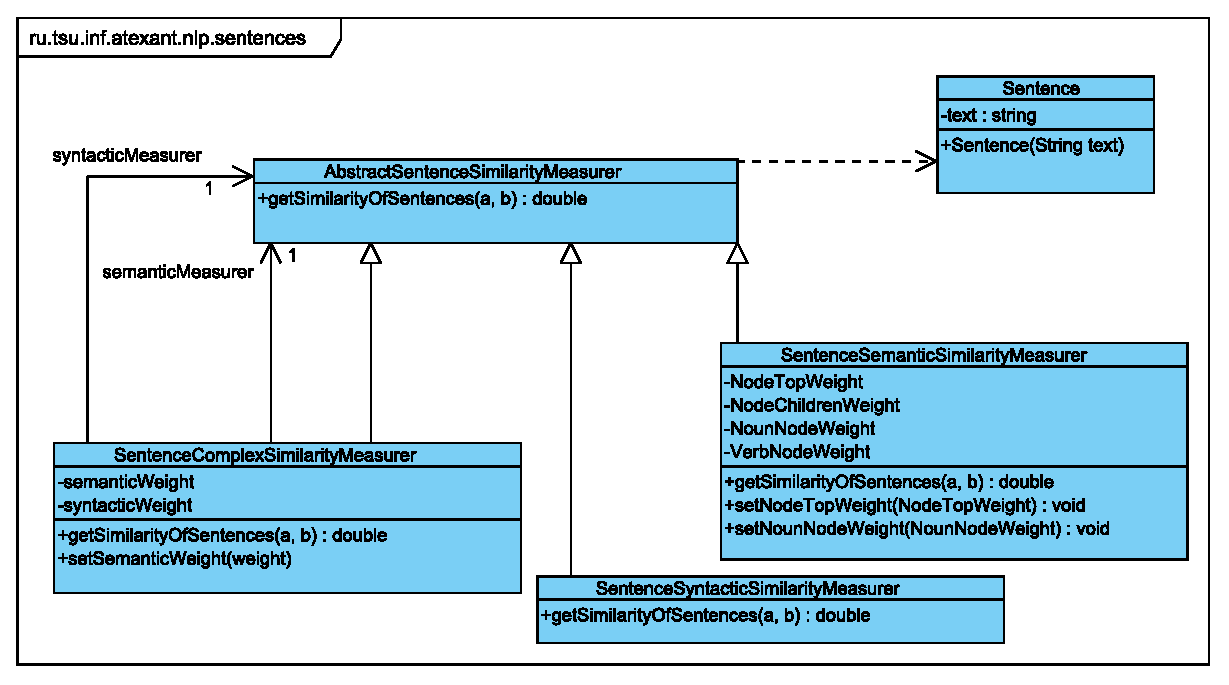
\includegraphics[scale=0.6]{eps/ru.tsu.inf.atexant.nlp.sentences.eps}
\caption{Диграмма классов пакета ru.tsu.inf.nlp.sentences}
\label{uml:ru.tsu.inf.atexant.nlp.sentences}
\end{center}
\end{figure}

%%По идее здесь нужно упомянуть, что использовались материалы, написанные для курсовой Валентины?

В~связи с~необходимостью проводить тестирование разных реализаций алгоритмов
для выявления наиболее эффективных из~них было принято решение выделить интерфейс
``AbstractSentenceSimilarityMeasurer''(рис. \ref{uml:ru.tsu.inf.atexant.nlp.sentences2}), 
каждая реализация которого содержит описание метода ``getSimilarity'',
призванного определить меру близости предложений, переданных ему в~качестве аргументов.
Сами предложения инкапсулированы в~объектах класса ``Sentence'', предоставляющих доступ
непосредственно к~их тексту, а также дереву зависимостей для каждого из~них.

\begin{figure}
\begin{center}
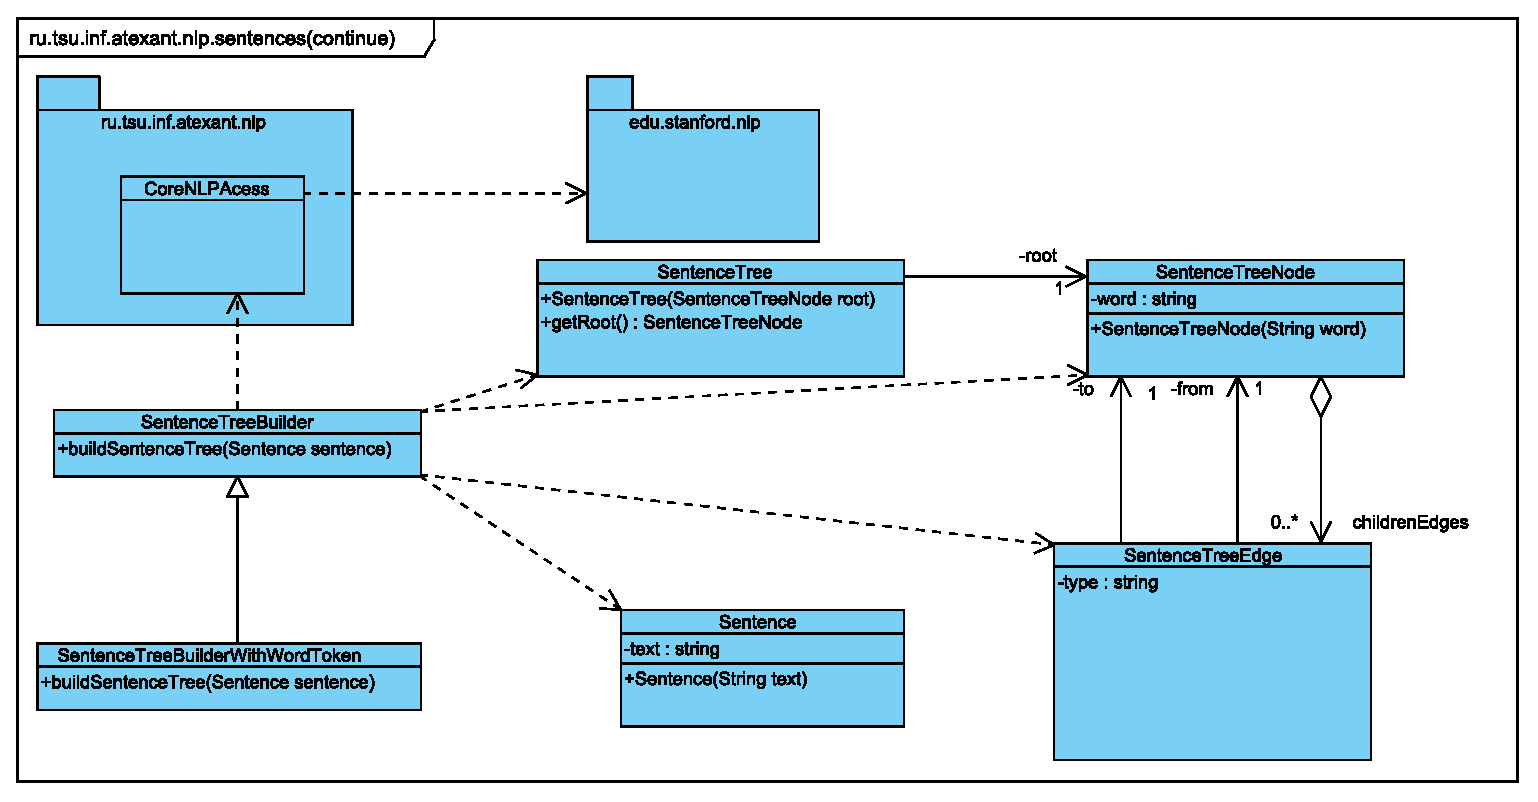
\includegraphics[scale=0.6]{eps/ru.tsu.inf.atexant.nlp.sentences(continue).eps}
\caption{Диграмма классов пакета ru.tsu.inf.atexant.nlp.sentences(Продолжение)}
\label{uml:ru.tsu.inf.atexant.nlp.sentences2}
\end{center}
\end{figure}

В~процессе реализации алгоритма были выделены классы ``SentenceSemanticSimilarityMeasurer'',
``SentenceSyntacticSimilarityMeasurer'' и ``SentenceComplexSimilarityMeasurer'':
первые два соответственно решают задачи, выделенные при~декомпозиции, описанные
в~разделах выше - оценивание семантической (см. \ref{sec:semantic_similarity}) 
и синтаксической близости (см. \ref{sec:syntactic_similarity}),
а третий ответственен за~объединение их результатов. 

Причем объекты этих классов
могут быть конфигурированы параметрами, определяющими весомость разных факторов
(в разделе выше они названы $\alpha_1,\alpha_2,\beta_1, \beta_2, \gamma_1, \gamma_2$).
Это позволяет оценить при запусках алгоритма то, как разные значения этих параметров влияют на~результат работы,
и выбрать оптимальные. Кроме того SentenceComplexSimilarityMeasurer может быть инициализирован 
другими реализациями AbstractSentenceSimilarityMeasurer, имеющими все тот~же смысл
измерителей семантической и синтаксической схожестей, что позволяет в~дальнейшем модифицировать алгоритм,
оставаясь при этом в~рамках того~же каркаса декомпозиции. 

Более детально реализацию алгоритма можно рассмотреть в~git-репозитории\cite{github},
обратив внимание на пакет ``ru.tsu.inf.atexant.nlp.sentence'',
расположенный в~соответствующем каталоге.

\subsection{Результаты}
В~рамках настоящей работы был реализован один из~алгоритмов определения схожести предложений.
Для~оценки его эффективности алгоритм был запущен на~тестовом наборе,
предложенном в~\cite{complexSim}. Этот набор представляет из~себя множество пар предложений,
каждое из которых является толькованием какого-то ``понятия'' (например, автомобиль - это самоходное транспортное средство),
причем степень близости описываемых ``понятий'' была оценена группой людей.

В таблице (см. \ref{app:sentence_similarity_table}) приведены усреденные оценки близости понятий данные людьми,
результаты вышеописанного алгоритма, запущенного для предложений-толкований этих понятий, 
а так~же значения отклонения оценок алгоритма от~оценок людей, 
представленное в~виде модуля разности этих величин.

Среднее значение отклонений результатов работы алгоритма от~оценок данных людьми равно $0.150915$,
что можно считать неплохим результатом с учетом узких для данного алгоритма мест,
которые присутствуют в~этом тестовом наборе, и о~которых будет сказано ниже. 
Наибольшее значение погрешности ($0.361794$) было получено для пары предложений:
\begin{itemize}
\item {
	A boy is a child who will grow up to be a man.
}
\item {
	A rooster is an adult male chicken.
}
\end{itemize}
где значение оценки, данной людьми, составляет $0.1075$, а результат алгоритма --- $0.469294$.
Такое расхождение между оценками людей и оценки-результата алгоритма может быть вызвано
следующими факторами:
\begin{enumerate}[a.]
\item {
При оценке люди отдают себе отчет в~том, что понятия ``мальчик'' и ``петух'', если и связаны,
то являются антонимичными, так как второе имеет значение ``взрослый цыпленок'', противоположное
значению понятия ``ребенок'', что в~итоге приводит к низкой величине оценки. 
Алгоритм наоборот даст более высокую оценку близости антонимам, чем словам,
совсем несвязанным друг с~другом. А в~данных предложениях присутствует
много пар слов, имеющих близкое в~этом смысле значение, что завышает итоговую оценкую.
}
\item {
Оценивая семантическую - более весомую часть, алгоритм учитывает только отдельные вершины
с их потомками, и в~этом примере алгоритмом было обнаружено много схожих пар.
}
\end{enumerate}

В~качестве еще одного примера работы алгоритма был реализован
модуль поиска предложений в~определенной статье Wikipedia.
Его суть состоит в~том, что он сравнивает введенное пользователем предложение
со всеми предложениями, содержащимися в~выбранной им же статье, сортирует их по~убыванию
схожести с~предложением пользователя и выводит на экран результаты работы.
В~приложении к~статье можно найти пример работы полученного алгоритма со~статьей ``Alchemy''.
Для проверки было выбрано предложение из~этой же~статьи:

\textit{"The best known goals of the alchemists were the transmutation of common metals into Gold or Silver, and the creation of a "panacea," a remedy that supposedly would cure all diseases and prolong life indefinitely; and the discovery of a universal solvent."}

Для проверки качества работы алгоритма оно было изменено:

\textit{"The most famous targets of the alchemist's is the transformation of common metals into gold, and making of a magic remedy named panacea".}

В~результате запуска алгоритма (см. \ref{app:sentence_wikipedia_search}) в~качестве наиболее похожего 
было выбрано исходное предложение со~значением меры близости $0.334027866$.

Таким образом задачу поиска предложения алгоритм выполнил, однако значение меры близости
по мнению автора в~данном случае занижено.

Учитывая обнаруженные таким образом недостатки, а так~же замечания, 
сделанные во~время анализа алгоритма в~разделе \ref{sec:complex_algorithm_analysis}, автором были
выдвинуты следующие предложения по~улучшению данного алгоритма:
\begin{itemize}
\item{
Во-первых для~улучшения среднего значения отклонений результатов следует
при~оценке семантической близости учитывать расстояние от~корня дерева зависимостей
до~сравниваемых вершин. Для этого необходимо отойти от~предложенной авторами модели с~векторным пространством,
так~как в~ней не предусмотрены разные веса для~разных ее компонент при~оценке близости векторов, взятой как косинус угла между ними.
}
\item{
Еще одним улучшением было~бы использование более эффективного алгоритма для установления
степени схожести деревьев зависимостей, это могло~бы позволить более точно сравнивать
синтаксическую структуру предложений. 
}
\item{
Одним из~недостатков реализованного метода в~случае применения его для~поиска 
является то, что он предназначен для~введения меры эквивалентности предложений, когда для~задач поиска
более удобной формой является мера вхождения одного предложения в~другое, позволяющая найти предложение только по~его части.
Для его устранения в~семантической части векторное пространство нужно строить только на основе базиса искомого предложения,
а в~синтаксической в~формуле, дающей результат, в~качестве знаменателя использовать мощность множества,
соответсвующего искомому предложению.
}
\end{itemize}


